\documentclass[aspectratio=169]{beamer}

% \usetheme{Frankfurt}
\usetheme{Warsaw}

\usecolortheme{seahorse}
\usecolortheme{rose}

\setbeamertemplate{footline}[frame number]
\setbeamertemplate{navigation symbols}[vertical]

% ****************************************************************
% Nikhil's defs

% ----------------
% EMPTY BOXES OF VARIOUS WIDTHS, FOR INDENTATION
\newcommand{\hm}{\hspace*{1em}}
\newcommand{\hmm}{\hspace*{2em}}
\newcommand{\hmmm}{\hspace*{3em}}
\newcommand{\hmmmm}{\hspace*{4em}}

\newcommand{\tinytt}{\tiny\tt}
\newcommand{\scripttt}{\scriptsize\tt}

\setcounter{section}{10}

% ****************************************************************

\title{Installation instructions}

\subtitle{for tutorial: ``A Tour of the RISC-V ISA Formal Specification''}

\author{RISC-V Foundation ISA Formal Spec Technical Committee}

\date{At RISC-V Summit, San Jose \\ December 12, 2019}

% ****************************************************************
% ****************************************************************
% ****************************************************************

\begin{document}

% ----------------
\begin{frame}
  \titlepage
\end{frame}


% ----------------
\begin{frame}
  \frametitle{Outline}
  \tableofcontents
\end{frame}

% ****************************************************************

\section{About this slide deck}
% \addcontentsline{toc}{section}{About this slide deck}

% ----------------

\begin{frame}
  \frametitle{About this slide deck}

  \scriptsize

  This is a standalone slide deck that accompanies the main slide deck
  for the tutorial: ``A Tour of the RISC-V ISA Formal Specification'',
  first presented at the RISC-V Summit, December 12, 2019, San Jose.

  \vspace*{1ex}

  We recommend taking either Step A, or Steps A and B, depending on
  your objectives, in advance of the tutorial.

  \begin{block}{Step A: If you just want to learn how to \emph{read and consult the spec}}
    This merely git-clones a certain repo which contains the SAIL source code
    for the RISC-V ISA Formal Spec.
  \end{block}

  \begin{block}{Step B: If you also want to learn how to \emph{execute the spec}}

    This will compile a RISC-V ISA simulator from the SAIL formal
    spec, which you can use to execute:

    \begin{itemize}
    \item The standard suite of RISC-V ISA tests
    \item The standard RISC-V Compliance Test suite
    \item RISC-V ELF binaries that you create from other source codes
    \end{itemize}
  \end{block}

\end{frame}

% ****************************************************************

\section{Installation for reading the spec}

% ----------------
\begin{frame}
  \frametitle{Installation Overview}

  \centering
  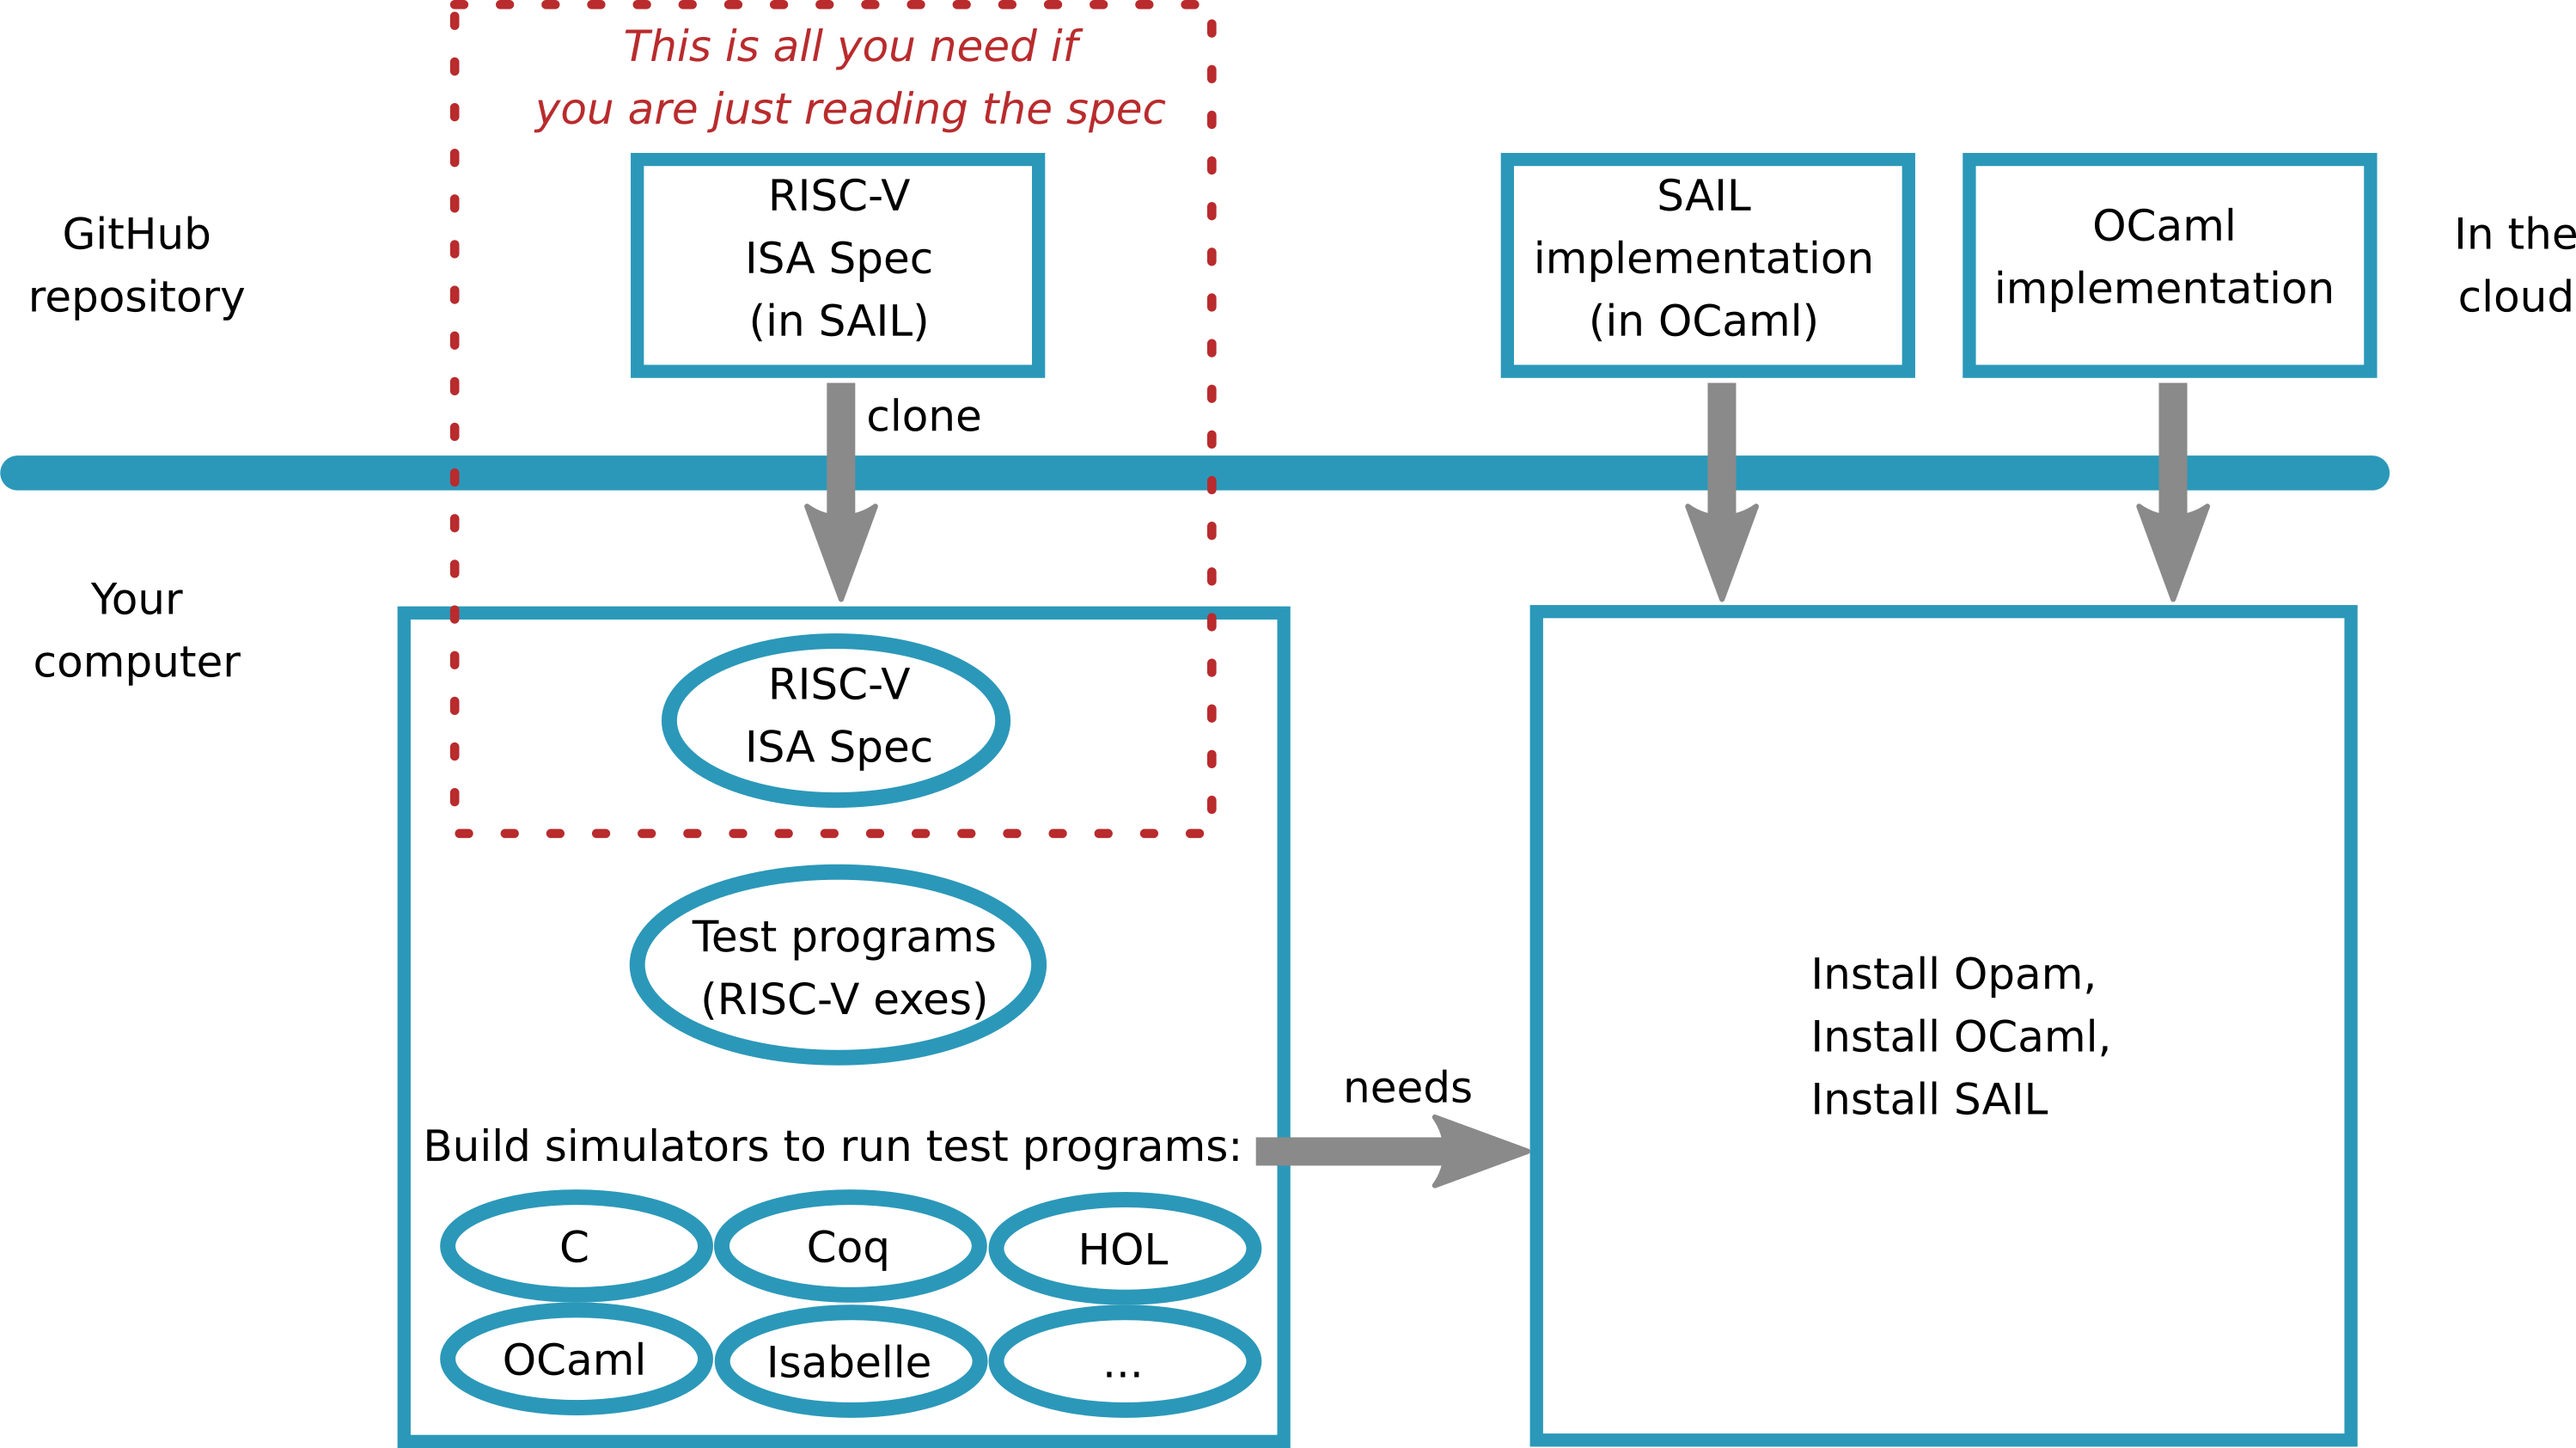
\includegraphics[height=2.4in]{Figures/Fig_Installation_Overview.png}
\end{frame}


% ================================================================

\subsection{Cloning the SAIL RISC-V ISA Formal Spec}

% ----------------
\begin{frame}
  \frametitle{Step A Installation: Cloning the SAIL RISC-V ISA Formal Spec}

  \begin{block}{Just one step:}
    {\scripttt\hm{}\$ git clone https://github.com/rems-project/sail-riscv}
  \end{block}

  \begin{block}{What you get:}
    {\scripttt\hm{}\$ sail-riscv} \\
    {\scripttt\hm{}\$ tree -d} \\
    {\scripttt\hm{}|-- ...} \\
    {\scripttt\hm{}|-- model/} \hspace{5em} \emph{This directory contains all the spec files}\\
    {\scripttt\hm{}|-- ...} \\
  \end{block}

  That's all you need, for just reading and consulting (not executing) the spec!

\end{frame}

% ****************************************************************

\section{Installing for building executable version of the spec}

% ----------------
\begin{frame}
  \frametitle{Step B Installation: to create an executable version of the spec}

  \begin{block}{Safety net, in case things go wrong:}
    \scriptsize
    The instructions in these slides are collected here from various
    sources for your convenience. In case of trouble, the original
    full instructions can be found at:

    \begin{itemize}

      \item Installing Opam: \\
        {\scripttt\hm https://opam.ocaml.org/doc/Install.html}

      \item Installing Ocaml for SAIL, and installing SAIL: \\
        {\scripttt\hm https://github.com/rems-project/sail/wiki/OPAMInstall}

    \end{itemize}
  \end{block}

  \begin{block}{OS requirements}
    \scriptsize
    These instructions are given for Debian/Ubuntu Linux.  Alternatives:
    \begin{itemize}
      \item You could install a virtual machine running Debian/Linux and follow these instructions


      \item OCaml and SAIL will also install on other OSes. Wherever
        you see ``{\tt apt get}'' here, which is the standard package
        manager for Debian/Ubuntu, please substitute the package
        manager for your OS.  The websites mentioned under ``Safety
        net'' above may also have more information for other OSes.

    \end{itemize}
  \end{block}

\end{frame}

% ----------------
\begin{frame}
  \frametitle{Installation Overview}

  \centering
  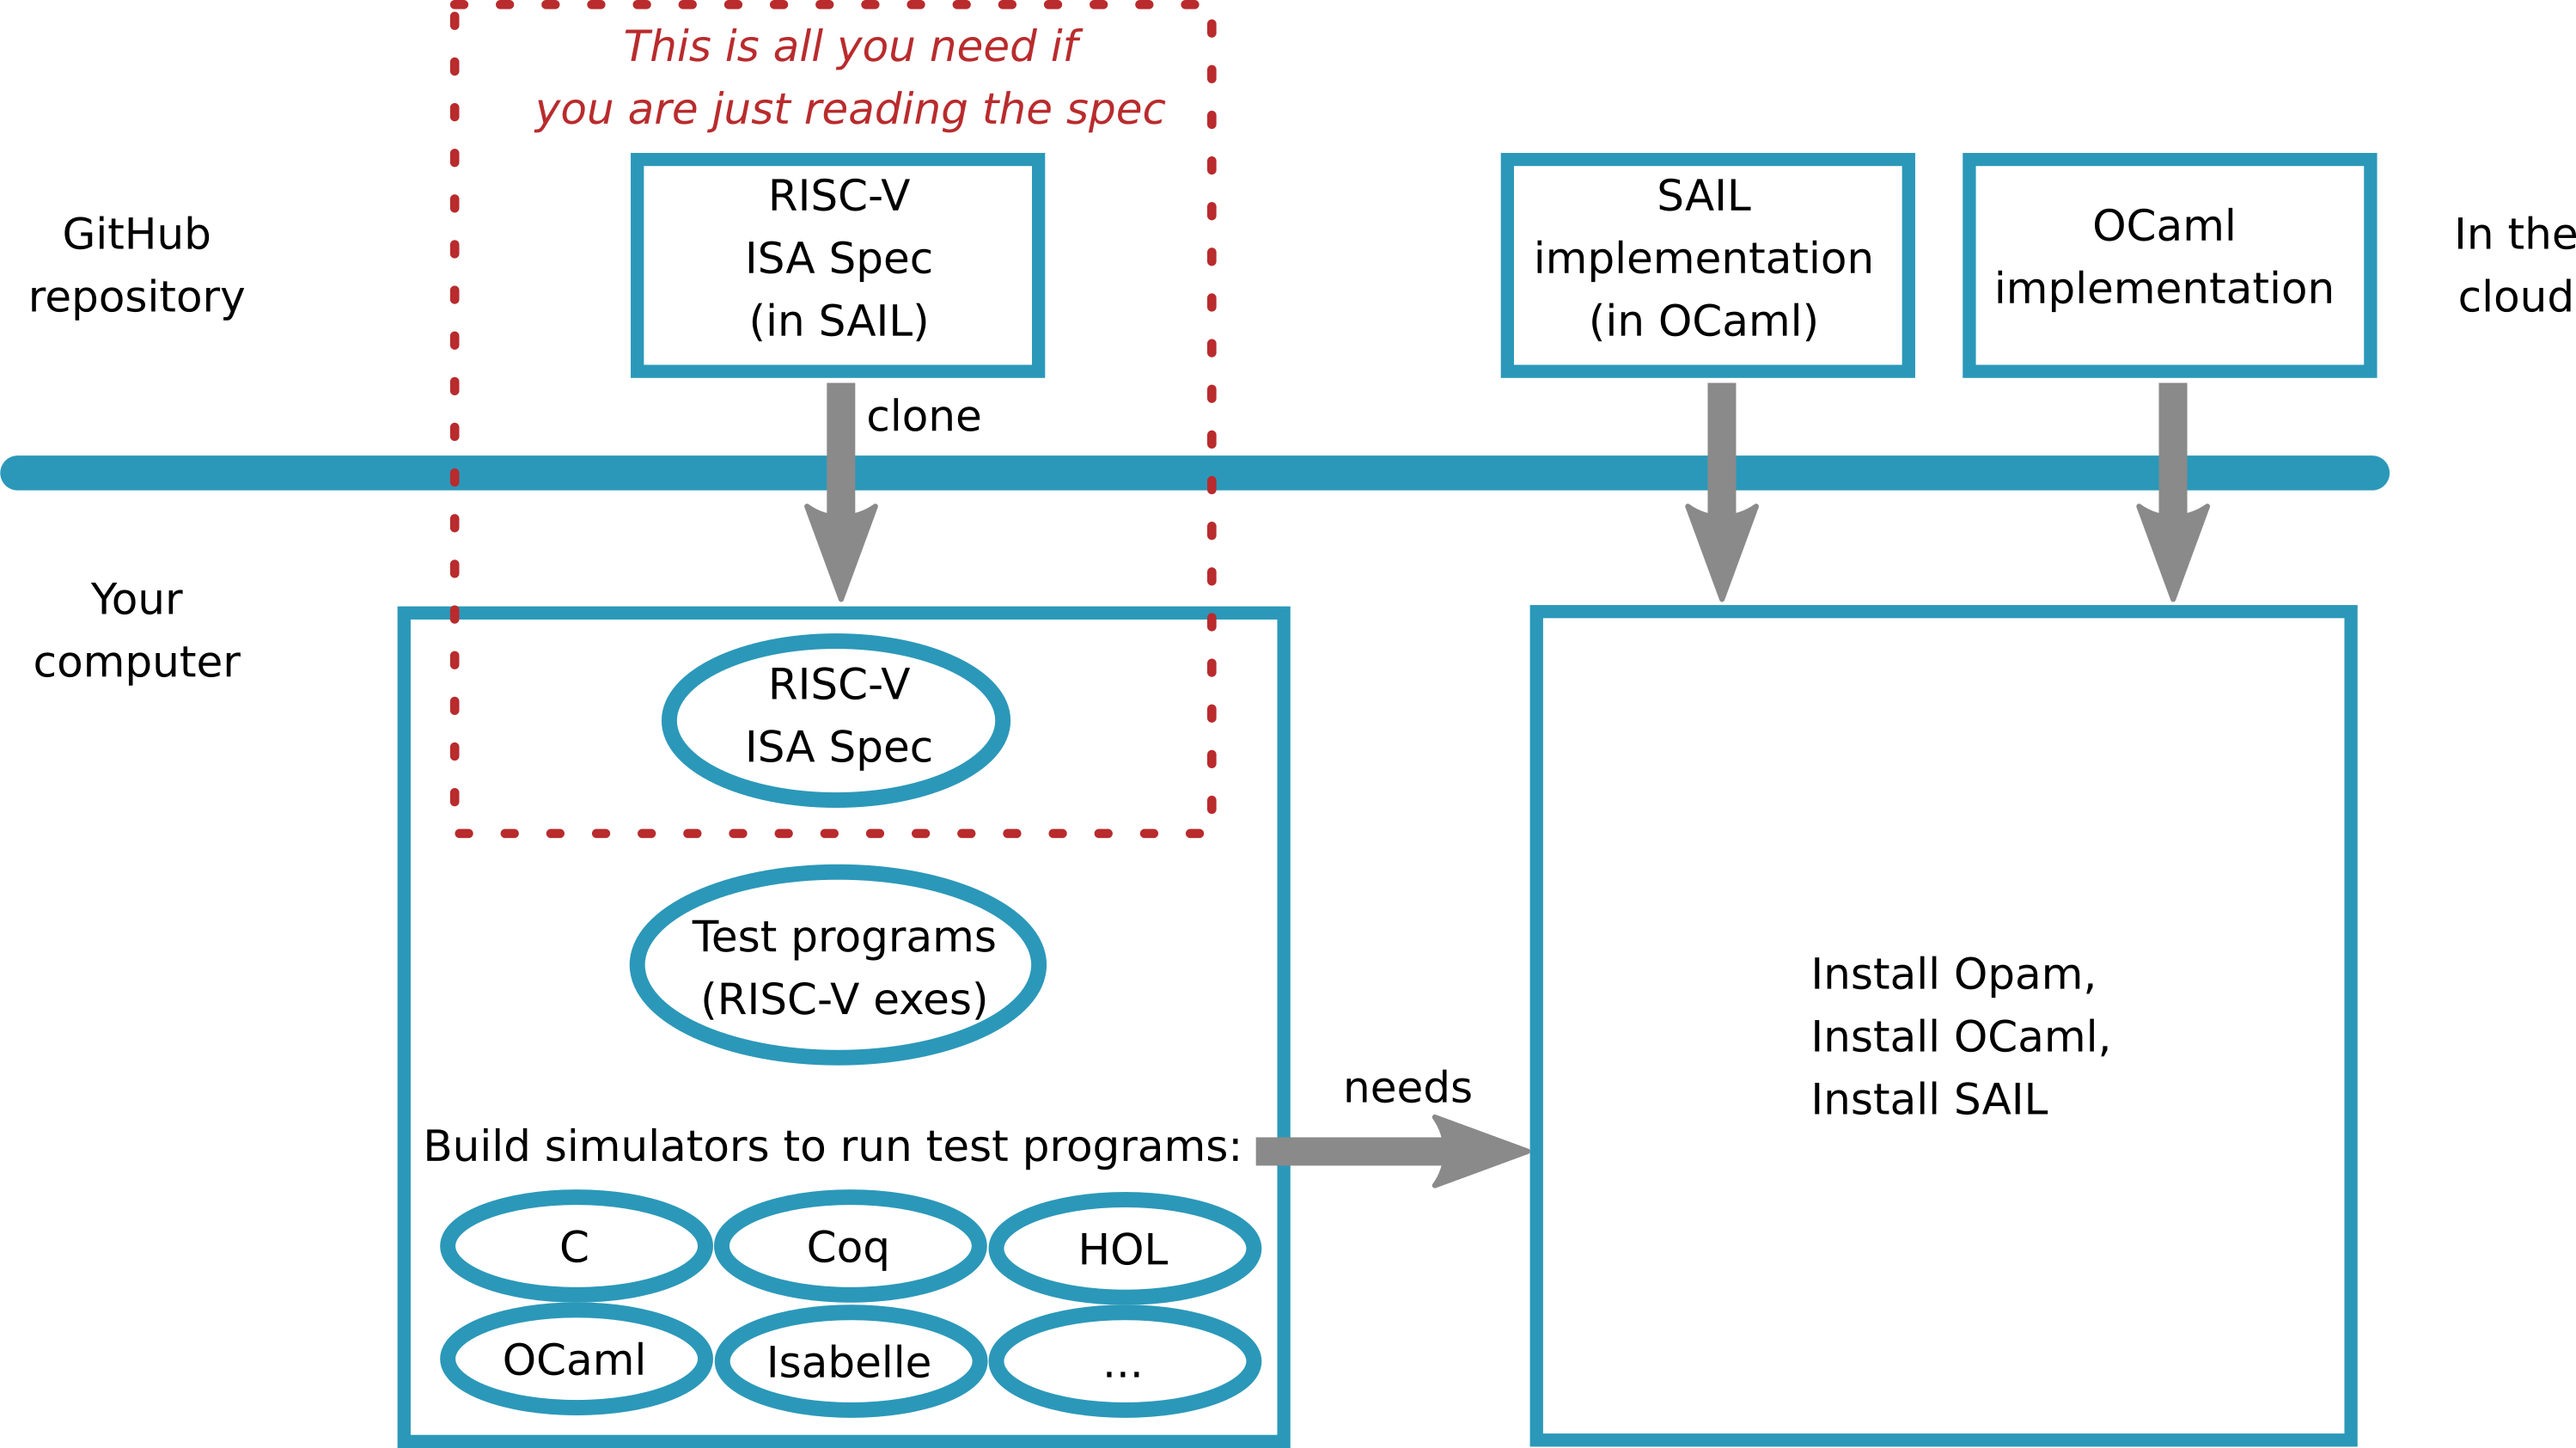
\includegraphics[height=2.4in]{Figures/Fig_Installation_Overview.png}
\end{frame}


% ================================================================

\subsection{Installing Opam}

% ----------------
\begin{frame}
  \frametitle{Step B.1: Installing Opam, the package manager for OCaml}

  Reminder: Step B is not necessary if you're only reading and
  consulting the spec.

  It's necessary to build simulator(s) from the SAIL RISC-V ISA Formal
  Spec that can execute RISC-V binaries.

  \vspace*{2ex}

  Use either of the following methods to install Opam:

  \begin{block}{Step B.1 Method 1: Use curl to get an install script and run it directly:}
    Install curl if you don't already have it: \\
    {\scripttt\hm{}\$ sudo apt-get install curl} \\
    Install Opam: \\
    {\scripttt\hm{}\$ sudo sh <(curl -sL https://raw.githubusercontent.com/ocaml/opam/master/shell/install.sh)}
  \end{block}
\end{frame}

% ----------------
\begin{frame}
  \frametitle{Installing Opam (contd.)}

  \begin{block}{Step B.1 Method 2: Download the install script and run it explicitly}
    Download {\tt install.sh} from the above web link, and run it: \\
    {\scriptsize
      \hm{}{\tt \$} ... \emph{download} \hm {\tt https://raw.githubusercontent.com/ocaml/opam/master/shell/install.sh}} \\
    {\scripttt
      \hm{}\$ sudo sh install.sh \\
      \hm{}\#\# Downloading opam 2.0.5 for linux on x86\_64... \\
      \hm{}\#\# Downloaded. \\
      \hm{}\#\# Where should it be installed ? [/usr/local/bin] \\
      \hm{}\#\# opam 2.0.5 installed to /usr/local/bin \\
      \hm{}\#\# Run this script again with '--restore ' to revert.}
  \end{block}

  \begin{block}{Step B.1: Verify successful opam installation (after using either method above)}
    {\scripttt
      \hm{}\$ which opam \\
      \hm{}/usr/local/bin/opam \\
      \hm{}\$ opam --version \\
      \hm{}2.0.5 }
  \end{block}

\end{frame}

% ================================================================

\subsection{Installing OCaml using Opam}

% ----------------
\begin{frame}
  \frametitle{Step B.2: Installing OCaml using Opam}
  Once Opam is installed, you can use it to install OCaml and SAIL.  First, OCaml:

  \begin{block}{Step B.2: Installing OCaml, and verifying we've got it}
    {\scripttt
      \hm{}\# Environment setup \\
      \hm{}\$ opam init \\
      \hm{}\$ eval `opam env` \\
      \hm{}\# Install specific version of OCaml \\
      \hm{}\$ opam switch create ocaml-base-compiler.4.06.1 \\
      \hm{}\$ eval `opam config env` \\
      \hm{} \\
      \hm{}\# Verify we've got it \\
      \hm{}\$ which ocaml \\
      \hm{}/home/nikhil/.opam/ocaml-base-compiler.4.06.1/bin/ocaml \\
      \hm{}\$ ocaml -version \\
      \hm{}The OCaml toplevel, version 4.06.1
    }
  \end{block}

  {\footnotesize Note: 4.06.1 is not the latest version of OCaml,
    but it is known to be suitable for SAIL (it is the version used during CI of SAIL).}

\end{frame}

% ================================================================

\subsection{Installing SAIL using Opam}

% ----------------
\begin{frame}
  \frametitle{Step B.3: Installing SAIL using Opam}

  Some prerequisites: install certain libraries needed by SAIL (if not already installed on your system)

  \begin{block}{On Linux (Debian, Ubuntu, ...)}
    \scripttt
    \begin{tabular}{l}
      \$ sudo apt-get install build-essential libgmp-dev z3 m4 pkg-config zlib1g-dev \\
      \$ sudo apt-get install device-tree-compiler \hmmm {\it Needed by OCaml-based simulator}
    \end{tabular}
  \end{block}

  \begin{block}{Homebrew (Mac OS)}
    \scripttt
    \begin{tabular}{l}
      \$ brew install gmp z3
    \end{tabular}
  \end{block}

\end{frame}

% ----------------

\begin{frame}
  \frametitle{Step B.3 (contd.): Installing SAIL using Opam}

  \begin{block}{Set up opam so it knows where to get SAIL}
    {\scripttt
      \hm{}\$ opam repository add rems https://github.com/rems-project/opam-repository.git
    }
  \end{block}

  \begin{block}{Install SAIL, and verify we've got it}
    {\scripttt
      \hm{}\$ opam install sail \\
      \hm{} \\
      \hm{}\# Verify we've got it \\
      \hm{}\$ which sail \\
      \hm{}/home/nikhil/.opam/ocaml-base-compiler.4.06.1/bin/sail \\
      \hm{}\$ sail --help \\
      \hm{}Sail 0.11 (sail2 @ opam) \\
      \hm{}usage: sail <options> <file1.sail> ... <fileN.sail> \\
      \hm{} \\
      \hm{}  -o <prefix>                              select output filename prefix \\
      \hm{}  -i                                       start interactive interpreter \\
      \hm{}  ...
    }
  \end{block}

\end{frame}

% ================================================================

\subsection{Building RISC-V simulator(s) from the SAIL spec}

% ----------------

\begin{frame}
  \frametitle{Step B.4: Building RISC-V simulator(s) from the SAIL spec}

  A simulator can be used to execute RISC-V binaries.

  \begin{block}{Step B.4: Building RISC-V simulator(s):}
    \scriptsize
    \begin{tabular}{ll}
      \tt \$ cd sail-riscv \hmmm & \emph{i.e.,} be in the git-cloned directory \\
      \tt \$ make
    \end{tabular}
  \end{block}

  \begin{block}{Creates the following (RV64 is the default):}
    \scriptsize
    \begin{tabular}{ll}
      \tt c\_emulator/riscv\_sim\_RV64            & Generates a C simulator and compiles it \\
      \tt ocaml\_emulator/riscv\_ocaml\_sim\_RV64 & Generates an OCaml simulator and compiles it \\
    \end{tabular}

    ... and Coq, Isabelle and HOL4 models in other directories ...
  \end{block}

  \begin{block}{You can also create corresponding RV32 simulators:}
    {\scripttt
      \hm{}\$ ARCH=RV32 make}
  \end{block}

\end{frame}

% ****************************************************************

\end{document}
